%%%%%%%%%%%%%%%%%%%%%%%%%%%%%%%%%%%%%%%%%%%%%%%%%%%%%%%%%%%%%%%%%%%%%%%%%%%%%%%
%
%2345678901234567890123456789012345678901234567890123456789012345678901234567890
%        1         2         3         4         5         6         7        8

%\documentclass[letterpaper, 10 pt, conference]{ieeeconf}  
\documentclass[a4paper, 10pt, conference]{ieeeconf}      
                                                          



% The following packages can be found on http:\\www.ctan.org
\usepackage{graphics} % for pdf, bitmapped graphics files
\usepackage{epsfig} % for postscript graphics files
\usepackage{mathptmx} % assumes new font selection scheme %installed
\usepackage{times} % assumes new font selection scheme installed
\usepackage{amsmath} % assumes amsmath package installed
\usepackage{amssymb}  % assumes amsmath package installed


\title{\LARGE \bf
Amplificador de Eletrocardi\'ografo} 


\author{Fernanda Amaral$^{1}$ ,Gabriel Miranda$^{2}$ e 
Luiz Fernando Araujo$^{3}$ 
}


\begin{document}



\maketitle
\thispagestyle{empty}
\pagestyle{empty}


%%%%%%%%%%%%%%%%%%%%%%%%%%%%%%%%%%%%%%%%%%%%%%%%%%%%%%%%%
%%%%%%%%%%%%%%%%%%%%%%%
\begin{abstract}
O projeto descrito a seguir teve como objetivo o estudo e 
a implementa\c c\~ao de um amplificador de eletrocardi
\'ografo. O eletrocardiograma (ECG) \'e um procedimento 
no qual os impulsos el\'etricos do cora\c c\~ao s\~ao 
amplificados e interpretados por um certo per\'iodo de 
tempo. Eletrocardi\'ografo, tamb\'em conhecido como ECG 
\'e o aparelho que realiza as medi\c c\~oes desses 
impulsos el\'etricos. O relat\'orio a seguir tem por 
finalidade explicar o funcionamento do ECG, desde o 
batimento do cora\c c\~ao at\'e a medi\c c\~ao e 
implementa\c c\~ao realizada. Ser\'a explicado a fun\c c
\~ao dos amplificadores utilizados e a maneira encontrada 
para que haja uma diminui\c c\~ao nos ru\'idos captados 
pelo sistema. O circuito presente nesse relat\'orio \'e 
baseado no modelo criado e implementado pela Texas 
Instruments (TI).



\end{abstract}

\section{INTRODU\c C\~ AO}


As atividades el\'etricas das c\'elulas humanas se d\~ao 
de diversas formas, 
sendo elas 
qu\'imicas, mec\^ anicas, t\'ermicas, luminosas e el\'etricas. O fen\^ omeno 
da 
atividade el\'etrica nos tecidos vivos se d\'a em n\'ivel 
celular, dependendo 
estritamente da membrana celular. Na maioria das c\'elulas foi detectado uma 
diferen\c ca de potencial el\'etrico entre o citoplasma e 
o exterior das c\'elulas. 
Esta diferen\c ca de potencial \'e chamada de Potencial 
de Membrana.
As cargas el\'etricas, capazes de conduzir eletricidade 
pelo corpo humano, s\~ao 
encontradas nos \'ions de compostos dissociados em meio 
aquoso, que est\~ ao 
dentro e 
fora das c\'elulas. Assim, o potencial de membrana se d\'a pela distribui\c 
c\~ ao 
desigual desses \'ions nos dois lados da membrana, 
fazendo com que a 
membrana atue como 
um capacitor, armazenando energia. Quando temos alguma 
perturba\c c\~ao, a c\'elula sai 
do repouso el\'etrico e muda seu valor. Rapidamente, a c
\'elula volta a 
estabelecer seu potencial de membrana. Esse processo tem 
suas fases, chamadas de despolariza
\c c\~ao e repolariza\c c\~ao, e entre elas, por meio de 
correntes el\'etricas (i\^onicas), cria-se um Potencial 
de A\c c\~ao. Esse potencial \'e, basicamente, a altera\c 
c\~ao r\'apida na polaridade das c\'elulas, onde seu 
interior fica positivo e o exterior negativo, e retornam 
ao normal. Esse processo ocorre na casa dos milissegundos. A 
imagem a seguir exemplifica o potencial de a\c c\~ ao e a 
polaridade das c\'elulas. 
\begin{figure}[!htb]
\centering
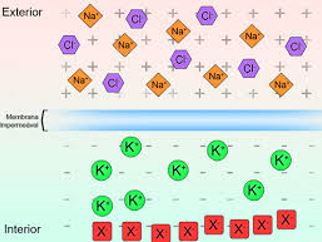
\includegraphics[width = 6cm, height = 6cm]{figura1}
\caption{Polaridade das c\'elulas.}
\end{figure}
\begin{figure}[!htb]
\centering
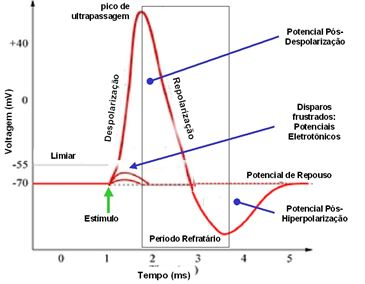
\includegraphics[width = 6cm, height = 6cm]{figura2}
\caption{Potencial de a\c c\~ao}
\end{figure}

O cora\c c\~ ao � um \' org\~ ao formado por musculatura 
estriada 
card
\'iaca, seu tamanho \'e aproximado ao tamanho de um punho 
adulto 
fechado. \'E composto por dois sistemas de bombeamento 
independentes, 
posicionados um do lado direito e outro do lado esquerdo. 
Cada um 
desses sistemas \'e composto por duas c�maras, denominadas 
\'atrios e 
ventr\'iculos. Como sabemos, a fun��o do cora\c c\~ ao \'e 
bombear 
sangue rico em oxig\^enio para todas as c\'elulas do corpo 
humano.
Devido ao potencial de a\c c\~ao, descrito no t\'opico anterior, 
as c
\'elulas card\'iacas t\^em condi\c c\~oes de produzir atividade 
el
\'etrica. O processo de contra\c c\~ao e relaxamento do cora\c c
\~ao 
\'e  organizado e iniciado por um impulso el\'etrico, que \'e o 
potencial de a\c c\~ao propagado c\'elula a c\'elula, atrav\'es 
do 
\'org\~ao em quest\~ao. Existem, em nossos cora\c c\~oes, c
\'elulas 
especificas com a fun\c c\~ao de formar, espontaneamente, seus 
potenciais de a\c c\~ao, gerando, assim, o batimento do cora\c c
\~ao. 
Essas c\'elulas s\~ao conhecidas como c\'elulas marcapasso pois 
iniciam o batimento e controlam a frequ\^encia do cora\c c\~ao. 
Esse 
tipo de c\'elula \'e encontrado no n\'o sinoatrial, localizado na 
parede atrial direita. Existem ainda outras c\'elulas que t\^em 
fun\c 
c\~ao marcapasso e assim, formam tecidos especializados em gera\c 
c
\~ao e condu\c c\~ao el\'etrica. Al\'em do n\'o sinoatrial, temos 
ainda o n\'o atrioventricular, o m\'usculo atrial, fibras de 
Purkinje, 
feixes de His e seus ramos e o m\'usculo ventricular. Na figura a 
seguir, mostra-se a localiza\c c\~ao de cada elemento citado na 
frase 
anterior.
\begin{figure}[!htb]
\centering
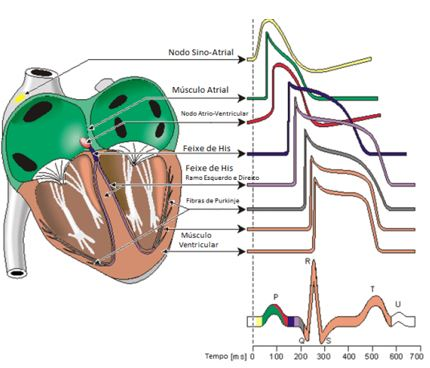
\includegraphics[width = 6cm, height = 6cm]{figura3}
\caption{Superposi\c c\~ao dos impulsos el\'etricos gerados e 
localiza\c c\~ao das partes geradoras.}
\end{figure}

Os impulsos, que se iniciam no n\'o sinoatrial, geram a forma de 
onda 
bastante conhecida, vista na Figura 3. Esses impulsos se propagam 
pelo 
\'atrio, promovendo a s\'istole atrial, que corresponde � onda P 
do 
eletrocardiograma. Ao atravessar o n\'o atrioventricular, os 
impulsos 
chegam ao sistema de condu\c c\~ao ventricular, onde a corrente 
de s\'odio 
\'e elevada. Isso faz com que a distribui\c c\~ao desse impulso 
seja 
ordenada. Assim, temos a s\'istole ventricular, que corresponde 
\`a onda QRS 
do eletrocardiograma. Ap\'os isso, ocorre a repolariza\c c\~ao 
dos \'atrios 
e ventr\'iculos. Com isso, o potencial de a\c c\~ao se encerra. 
Essa etapa 
de repolariza\c c\~ao corresponde \`a forma de onda T do 
eletrocardiograma.

\section{ASPECTOS T\'ECNICOS DO CIRCUITO}
O projeto do circuito do Eletrocardi\'ografo consiste em:
\begin{enumerate}
\item Adquirir os sinais biopotenciais do corpo humano
\item Amplificar o sinal de entrada de baixa amplitude, at\'e que 
este 
esteja em um n\'ivel de tens\~ao reconhec\'ivel pelos aparelhos 
de medi\c c
\~ao
\item Filtrar apenas a banda de frequ\^encia \'util para o sinal 
do ECG (De 0,5 Hz a 30 Hz aproximadamente)
\end{enumerate}
O esquem\'atico abaixo ilustra cada etapa da constru\c c\~ao em 
blocos
\begin{figure}[!htb]
\centering
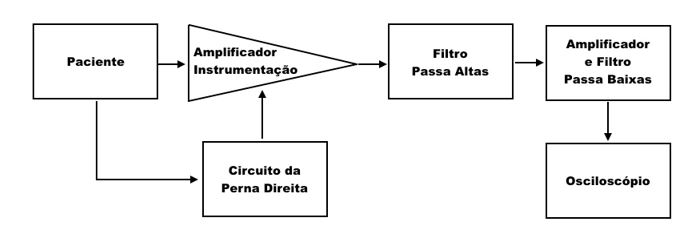
\includegraphics[width = 10cm, height = 7cm]{figura4}
\caption{Esquem\'atico da constru\c c\~ao do circuito}
\end{figure}

\subsection{Amplificador de instrumenta\c c\~ao}
Neste bloco foi utilizado o Circuito Integrado INA 118P da texas 
instruments de 
alta precis\~ao que amplifica com baixo ru\'ido os sinais vindos 
diretamente 
dos el\'etrodos ligados aos bra\c cos do paciente. O CI \'e 
ilustrado abaixo
\begin{figure}[!htb]
\centering
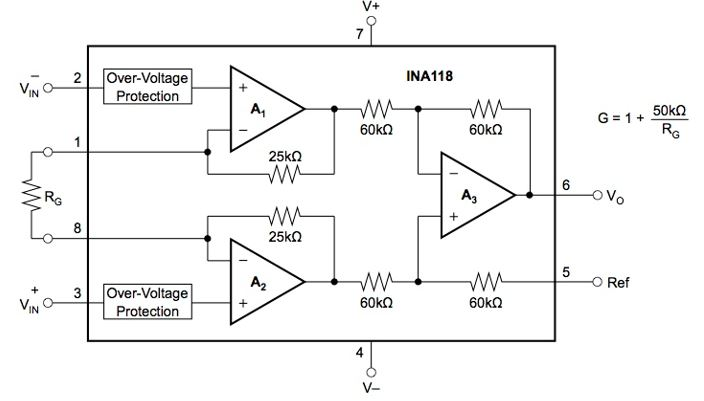
\includegraphics[width = 8cm, height = 6cm]{figura5}
\caption{Datasheet INA 118P}
\end{figure}

De acordo com o Datasheet do chip, o seu ganho � representado por
\begin{equation}
G = 1 + \frac{50k\Omega}{Rg}
\end{equation}
Em Rg, foram associados dois resistores de 2,7 kOhms (Por ser um 
valor 
comercial) encontramos o ganho dessa etapa do circuito: G = 
10,26.
\subsection{Circuito da Perna Direita}
O circuito da perna direita e\'e respons\'avel por inverter o 
sinal e injetar 
uma corrente na perna direita do paciente para causar uma 
interfer\^encia 
subtrativa, minimizando o ru\'ido em modo comum. O circuito 
utilizado nesta 
etapa foi encontrado no Datasheet do INA 118P na se��o de aplica
\c c\~oes. 
\begin{figure}[!htb]
\centering
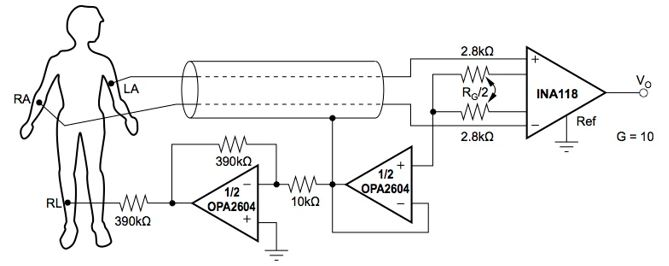
\includegraphics[width = 8cm, height = 5cm]{figura6}
\caption{Circuito a ser implementado}
\end{figure}

\subsection{Filtro Passa Altas}
Foi projetado o circuito de um filtro passa altas como o 
ilustrado a baixo, foi 
escolhido um valor comercial de capacit\^ancia: C = 330 nF.
\begin{figure}[!htb]
\centering
\includegraphics[width = 7cm, height = 6cm]{figura7}
\caption{Esquem\'atico filtro passa altas}
\end{figure}

Queremos obter uma frequ\^encia de corte de 0,1 Hz para eliminar 
as 
frequ\^encias inferiores n\~ao pertencentes \`a faixa do sinal 
bipotencial.
Queremos obter uma frequ\^encia de corte de 0,1 Hz para eliminar 
as 
frequ
\^encias inferiores n\~ao pertencentes \`a faixa do sinal 
bipotencial.
\begin{equation}
G = \frac{1}{2\pi RC}
\leftrightarrow
 R =\frac{1}{2\pi\cdot0.1\cdot330\cdot 10^{-9}}
 \cong 4.8M\Omega
\end{equation}
Foi escolhido o valor comercial de resistor de 4,7 MOhms.
\subsection{Filtro Passa Baixas}
Foi montado o circuito de um filtro passa baixas como o ilustrado 
a 
baixo.
\begin{figure}[!htb]
\centering
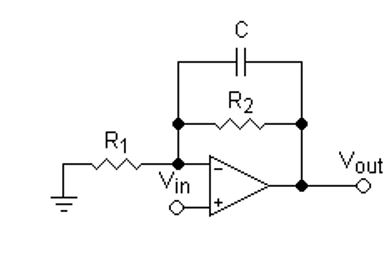
\includegraphics[width = 8cm, height = 6cm]{figura8}
\caption{Esquem\'atico filtro passa baixas}
\end{figure}

Queremos limitar a faixa superior de frequ�ncia com fc = 30 Hz, 
sabendo 
que
\begin{equation}
fc = \frac{1}{2\pi R_{2}C}
\end{equation}
Foi escolhido um valor de resist\^encia R2=100 kOhms. Mensurando 
o valor 
da capacit\^ancia, encontramos C = 53 nF. Dessa forma, foi 
utilizado o 
valor comercial mais pr\'oximo: C = 47 nF.
Para definir o ganho, fez-se uma an\'alise do sinal de entrada
\begin{figure}[!htb]
\centering
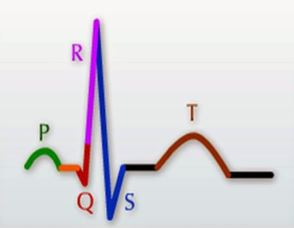
\includegraphics[width = 6cm, height = 6cm]{figura9}
\caption{Exemplo do sinal a ser obtido}
\end{figure}

Em condi\c c\~oes normais, as amplitudes das ondas dos sinais 
vitais s
\~ao
\begin{center}
\begin{tabular}{| l | l | l | l |}
\hline
Tens\~ao & Onda P & Complexo QRS & Onda T \\ \hline
Min & 0.1mV & 1mV & 0.2mV\\ \hline
Max & 0.3mV & 2mV & 0.3mV\\ \hline
  \end{tabular}
\end{center}

Como alimentamos o amplificador com � 2,5 V precisamos amplificar 
o 
sinal at� esse limite (no m\'aximo). A onda de maior amplitude 
\'e o 
Complexo QRS, com 2mV. Dessa forma, aplicando um ganho de 1000 no 
circuito todo teremos um sinal de sa\'ida com Vmax = 2V.
Na etapa do amplificador de instrumenta\c c\~ao foi aplicado um 
ganho de 
10. Ent\~ao, para alcan\c car um ganho total de 1000, vamos 
projetar 
esse bloco do circuito para ter um ganho igual a 100.
\begin{equation}
G =1 + \frac{R_{2}}{R_{1}} 
\leftrightarrow R_{1} = \frac{R_2}{100-1}
\end{equation}
Como j� temos R2=100 kOhms, descobrimos: R1=0,99 kOhms. O valor 
comercial mais pr�ximo para � R1=1 kOhm 
\subsection{Filtro Oscilosc\'opio}
A ideia desse projeto \'e a constru\c c\~ao de um Eletrocardi
\'ografo de 
f\'acil reprodu\c c\~ao e utiliza\c c\~ao port\'atil, sem a 
depend
\^encia dos aparelhos fixos do laborat\'orio. Assim, para a 
visualiza\c 
c\~ao das formas de onda de sa\'ida, foi utilizado um Ardu\'ino 
Nano que 
possui internamente um conversor Anal\'ogico Digital e possui f
\'acil 
conex\~ao com o computador para a plotagem do sinal.




\section{CONCLUS\~AO}
Com a realiza\c c\~ao do projeto apresentado, pode-se entender 
algumas  
das diversas aplica\c c\~oes do conte\'udo visto em sala de aula. 
Obteve-se o conhecimento necess\'ario para entender o 
funcionamento 
b\'asico da rela\c c\~ao de nosso corpo, c\'elulas e cora\c c
\~ao, com a 
eletricidade. Utilizou-se tamb\'em o conceito de filtros para 
realizar a 
filtragem dos ru\'idos presentes no circuito. At\'e ent~ao, 
obtivemos 
resultados promissores nas simula\c c\~oes e considera-se que o 
objetivo 
do projeto foi atingido.

\section*{AGRADECIMENTOS}
Gostar\'iamos de agradecer, pelo excelente apoio prestado, desde 
a aten\c c
\~ao para conosco at\'e a rapidez nas respostas de e-mails, aos 
professores 
Jo\~ao Luiz Azevedo de Carvalho, Doutor e  Ricardo Zelenovsky, 
Doutor.



\begin{thebibliography}{99}

\bibitem{c1} J. G. Webster,Medical Instrumentation Application and Design plastics (Book style with paper title and editor), 3rd ed. vol. 3.
\bibitem{c2} J. D. Irwin, Basic Enginnering Circuit Analysis (Book style), 10th ed. vol. 2.
\bibitem{c3} http://www.ti.com/
\bibitem{c4} http://www.datasheetcatalog.com/
\end{thebibliography}

\section*{ANEXOS}
Simula\c c\~oes computacionais. O circuito do Eletrocardi\'ografo \'e 
baseado na amplifica\c c\~ao do sinal de entrada e elimina\c c\~ao dos 
seus ru\'idos.
Como na entrada, foi colocada uma onda senoidal, esta mesma onda deve 
ser observada na sa\'ida, com uma amplitude maior.
Mesmo com a exist\^encia de filtros, n\~ao foram observados cortes na na onda de sa\'ida, porque a entrada se encontrava dentro da faixa de frequ\^encias desejada.
\begin{figure}[!htb]
\centering
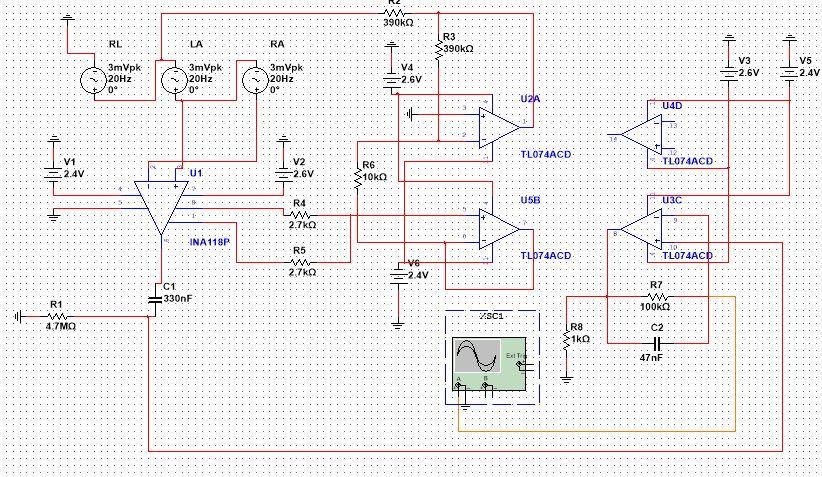
\includegraphics[width =15 cm, height = 10cm]{figura10}
\caption{Esquem\'atico do circuito montado}
\end{figure}
\begin{figure}[!htb]
\centering
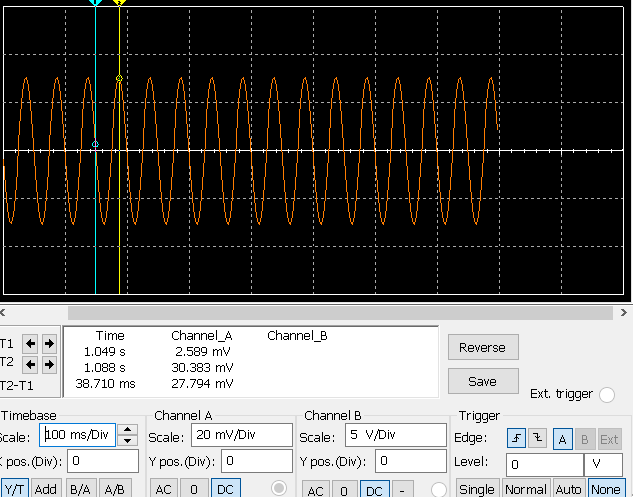
\includegraphics[width =15 cm, height = 10cm]{figura11}
\caption{Respostas das ondas obtidas na sa\'ida do circuito}
\end{figure}




\end{document}
